% Generated by book/tools/notebook_to_tex.py. Do not edit by hand.

\chapter[토크나이저 직접 학습 (Tokenizer Training)]{토크나이저 직접 학습 (Tokenizer Training)}

\label{ch:19}

\markboth{토크나이저 직접 학습 (Tokenizer Training)}{토크나이저 직접 학습 (Tokenizer Training)}

\chaptermeta{19_tokenizer_training/19_tokenizer_training.ipynb}{https://colab.research.google.com/github/yoon-gu/neuqes-101/blob/master/19_tokenizer_training/19_tokenizer_training.ipynb}{WordPiece와 WordLevel을 영어·한국어 코퍼스에서 직접 학습해 비교}



\index{1Tokenizer training@Tokenizer training}

\index{1WordPiece@WordPiece}

\index{1WordLevel@WordLevel}

\index{1tokenizers@tokenizers}

\index{1PreTrainedTokenizerFast@PreTrainedTokenizerFast}

\index{1vocab size@vocab\_size}

\index{1UNK token@UNK token}

\index{1BertPreTokenizer@BertPreTokenizer}

\index{1Whitespace@Whitespace}

\index{1TemplateProcessing@TemplateProcessing}

\index{0토크나이저 직접 학습@토크나이저 직접 학습}

\index{0워드피스@워드피스}

\index{0워드레벨@워드레벨}

\index{0어휘 수@어휘 수}

\index{0미등록 토큰@미등록 토큰}

\index{0교차 언어 적용@교차 언어 적용}

\index{0토큰 길이 분포@토큰 길이 분포}

\index{1Tokenizer@Tokenizer}

\index{1WordPieceTrainer@WordPieceTrainer}

\index{1WordLevelTrainer@WordLevelTrainer}

\index{1SPECIAL TOKENS@SPECIAL\_TOKENS}

\index{1PAD@[PAD]}

\index{1UNK@[UNK]}

\index{1CLS@[CLS]}

\index{1SEP@[SEP]}

\index{1MASK@[MASK]}

\index{1NFD@NFD}

\index{1Lowercase@Lowercase}

\index{1StripAccents@StripAccents}

\index{1NormSequence@NormSequence}

\index{1WordPieceDecoder@WordPieceDecoder}

\index{1Tokenizer from file@Tokenizer.from\_file}

\index{1tokenizer save@tokenizer.save}

\index{1cross language tokenization@cross-language tokenization}

\index{1unknown token rate@unknown token rate}

\index{1vocab sweep@vocab sweep}

\index{1subword token@subword token}

\index{1special token@special token}

\index{0직접 학습 토크나이저@직접 학습 토크나이저}

\index{0특수 토큰@특수 토큰}

\index{0서브워드@서브워드}

\index{0어절 단위@어절 단위}

\index{0어휘 스윕@어휘 스윕}

\index{0언어별 코퍼스@언어별 코퍼스}

\index{0한국어 코퍼스@한국어 코퍼스}

\index{0영어 코퍼스@영어 코퍼스}



\section{변화추적표}

\begin{booktable}{19장 변화추적표}{tab:ch19-01}
\begin{adjustbox}{max width=\textwidth}
\begin{tabular}{@{}llllll@{}}
\toprule
Ch & 모델 & 토크나이저 & 데이터 & Output & Loss \\
\midrule

17 & klue/bert-base & WordPiece (한국어, 사전학습) & KLUE-YNAT 합성 multi-label & \inlinecode{Linear(H,\ 7)} & \inlinecode{BCEWithLogitsLoss} \\
18 & klue/bert-base + 보조 & WordPiece (한국어, 사전학습) & KLUE-YNAT 합성 + 보조 라벨 & 메인(7) + 보조 & \texttt{BCEWithLogitsLoss\ +\ λ·L\_aux} \\
\textbf{19 \(\leftarrow\) 여기 (Phase 3 시작)} & --- (토크나이저 학습 전용) & \textbf{WordPiece + WordLevel} (둘 다 \emph{직접 학습}) & \textbf{Yelp text + NSMC text} & --- & --- \\
20 (다음) & 작은 BERT (직접, scratch) & \inlinecode{bert-base-uncased} 토크나이저 (가져옴) & Wikitext-103 (일반 도메인 위키) & MLM head & \inlinecode{CrossEntropyLoss} (masked) \\
\bottomrule
\end{tabular}
\end{adjustbox}
\end{booktable}

전체 장 표는 \href{https://github.com/yoon-gu/neuqes-101\#챕터별-변화추적표}{루트 README.md}를 참고하세요.

\textbf{Phase 3 의 위치} --- \ref{ch:19}장이 토크나이저 토대, \ref{ch:20}--\ref{ch:23}장은 그 위에 올린 작은 BERT 의 사전학습 + 분류. 단, \ref{ch:20}장부터는 \emph{학습 안정성} 을 위해 표준 사전학습 토크나이저 (\inlinecode{bert-base-uncased}, \inlinecode{klue/bert-base}) 를 그대로 가져와 씁니다. \ref{ch:19}장은 “토크나이저가 어떻게 학습되나” 를 \emph{경험} 하는 장.



\section{변경점: \ref{ch:18}장 대비}

\begin{booktable}{19장 변경점 요약}{tab:ch19-02}
\begin{adjustbox}{max width=\textwidth}
\begin{tabular}{@{}lll@{}}
\toprule
축 & \ref{ch:18}장 (한국어 auxiliary) & \ref{ch:19}장 (토크나이저 학습 전용) \\
\midrule

\textbf{이 장의 task} & 분류 (메인 multi-label + 보조) & \textbf{분류 아예 없음 --- 토크나이저 학습 그 자체가 결과물} \(\leftarrow\) \emph{유일한 변화} \\
모델 & \inlinecode{klue/bert-base} 파인튜닝 & 없음 \\
토크나이저 & 사전학습된 것 \emph{로드만} & \textbf{WordPiece + WordLevel 둘 다 \emph{직접 학습}} \\
데이터 & KLUE-YNAT 합성 multi-label + 보조 라벨 & Yelp text + NSMC text (라벨 무시, \emph{문장만} 사용) \\
Output / Loss & 메인 + 보조 + \(\lambda\) & 없음 (vocab + merge rules 가 산출물) \\
평가 metric & F1 / AUC / MAE & 토큰 길이 분포 / UNK 비율 / vocab 커버리지 \\
\bottomrule
\end{tabular}
\end{adjustbox}
\end{booktable}

\begin{quote}
\textbf{변경점 한 가지 원칙} --- Phase 2 (분류 task) 의 종착인 \ref{ch:18}장에서 \emph{task 자체} 가 토크나이저 학습으로 바뀝니다. 모델·loss·평가가 모두 사라지는 큰 전환이지만, 이건 \emph{축 자체} 가 바뀌는 Phase 경계라 자연스러움. Phase 3 의 다음 장부터 다시 모델 학습으로 돌아갑니다.
\end{quote}

\subsection{\texorpdfstring{왜 직접 학습하는가}{왜 토크나이저를 직접 학습해야 하나}}

새 도메인 (의료·법률·코드 등) 이나 새 언어로 BERT 를 사전학습할 때, 기존 토크나이저는 \emph{그 도메인의 어휘} 를 제대로 못 쪼갭니다. 예: 영어 토크나이저로 한국어를 처리하면 거의 모든 토큰이 \texttt{{[}UNK{]}} 가 됩니다. 도메인·언어에 맞춘 토크나이저를 직접 학습해야 모델이 \emph{압축된} 정보를 받을 수 있어요.



\section{알고리즘 노트}

이 장의 핵심 비교는 \emph{Loss 변화} 가 아니라 \textbf{토크나이저 알고리즘 변화} 입니다. 두 알고리즘은 분할 단위 자체가 다릅니다.

\subsection{WordLevel}

공백 단위로 단어를 잘라 그대로 vocab 에 등록. \emph{변형} 처리 없음.

\begin{itemize}
\tightlist
\item
  학습: 코퍼스에서 \emph{빈도 상위 N 단어} 를 골라 vocab 에 넣음. 나머지는 모두 \texttt{{[}UNK{]}}.
\item
  장점: 토큰화가 \emph{즉시} 이해 가능 (한 단어 = 한 토큰).
\item
  단점: vocab 밖 단어 = 전부 \texttt{{[}UNK{]}}. 영어처럼 굴절·합성이 많은 언어에서 OOV 가 폭증.
\end{itemize}

\subsection{WordPiece}

자주 등장하는 \emph{조각} 을 vocab 에 등록하고, 모르는 단어는 더 작은 조각으로 \emph{재귀적으로 쪼갬}. BERT 시리즈 (BERT / DistilBERT / KLUE-BERT) 가 이 알고리즘을 씁니다.

\begin{itemize}
\tightlist
\item
  학습: 처음에는 \emph{문자 단위 vocab} 부터 시작 \(\to\) likelihood 가 가장 많이 오르는 \emph{문자 쌍} 을 vocab 에 병합 \(\to\) vocab 목표 크기까지 반복.
\item
  처음 등장 토큰은 \inlinecode{playing}, 그 뒤를 잇는 조각은 \inlinecode{\#\#ing} 처럼 \inlinecode{\#\#} prefix.
\item
  장점: 모르는 단어도 \emph{작은 조각} 으로 쪼개 표현 가능 \(\to\) \texttt{{[}UNK{]}} 거의 안 남음.
\item
  단점: 짧은 단어 하나가 여러 조각으로 쪼개져 토큰 수가 늘어남.
\end{itemize}

\subsection{수치 예시}

학습된 두 토크나이저가 \emph{같은 문장} 을 어떻게 처리하나를 미리 감 잡기 --- 실제 결과는 §4 에서 직접 확인합니다.

\begin{booktable}{19장 손실 수치 예시}{tab:ch19-03}
\begin{adjustbox}{max width=\textwidth}
\begin{tabular}{@{}lll@{}}
\toprule
문장 & WordPiece (vocab 8K) & WordLevel (vocab 8K) \\
\midrule

\inlinecode{"the\ food\ was\ great"} (4 단어, 흔한 어휘) & 4 토큰 (1 단어=1 piece) & 4 토큰 (모두 vocab) \\
\inlinecode{"unforgettable\ experience"} (드문 어휘) & 5 토큰 (\inlinecode{un}, \inlinecode{\#\#forget}, \inlinecode{\#\#table}, \inlinecode{experience}) & 2 토큰 --- 단, \inlinecode{unforgettable} 이 vocab 밖이면 \texttt{{[}UNK{]}} \\
\inlinecode{"이\ 영화\ 정말\ 재미있어요"} (한국어) & 5-7 토큰 (조사·어미 분리) & 4 토큰 (어절 단위) --- 단, \inlinecode{재미있어요} vocab 밖이면 \texttt{{[}UNK{]}} \\
\bottomrule
\end{tabular}
\end{adjustbox}
\end{booktable}

핵심 관찰: \textbf{WordLevel 은 “단어가 vocab 에 있느냐 없느냐” 의 binary} --- 있으면 1 토큰, 없으면 \texttt{{[}UNK{]}}. \textbf{WordPiece 는 “얼마나 잘게 쪼갤지” 의 spectrum} --- 흔한 단어는 1 토큰, 드문 단어는 여러 조각.

\subsection{BERT와 WordPiece}

(1) \texttt{{[}UNK{]}} 토큰이 거의 안 생겨 모든 단어가 \emph{학습 가능} 한 표현으로 인코딩됨. (2) vocab 크기가 작아도 (BERT 30K, KLUE 32K) \emph{어휘 커버리지} 가 좋음. (3) 미세한 형태 차이 (\inlinecode{run}/\inlinecode{running}/\inlinecode{runs}) 가 \emph{공통 조각} 으로 묶여 표현 학습이 효율적.



\section{\texorpdfstring{토크나이저 노트}{토크나이저 노트}}

지금까지의 모든 장에서 마지막 자리를 차지하던 이 섹션이, 이번엔 장의 \emph{전체} 입니다.

\begin{itemize}
\tightlist
\item
  \textbf{\ref{ch:07}--\ref{ch:14}장}: 영어 WordPiece (\inlinecode{distilbert-base-uncased}, vocab 30K, 사전학습) 받아 쓰기.
\item
  \textbf{\ref{ch:15}--\ref{ch:18}장}: 한국어 WordPiece (\inlinecode{klue/bert-base}, vocab 32K, 사전학습) 받아 쓰기.
\item
  \textbf{\ref{ch:19}장 (지금)}: \emph{같은 WordPiece 알고리즘} + 단순 비교용 WordLevel 을 두 언어 코퍼스에서 \emph{직접} 학습.
\item
  \textbf{\ref{ch:20}장+}: 다시 표준 사전학습 토크나이저로 --- 단, \emph{이제는 그 안에서 무엇이 벌어지는지 알고} 사용.
\end{itemize}

같은 알고리즘이 \emph{언어가 바뀌면 어떻게 다른 결과} 를 내는지 (영어 vs 한국어), \emph{알고리즘이 바뀌면 어떻게 다른 결과} 를 내는지 (WordPiece vs WordLevel) --- 2\(\times\)2 비교가 이 장의 핵심.



\section{환경 준비}



\section{영어 코퍼스}

\inlinecode{yelp\_polarity} 의 train split 에서 5,000 문장만 sample. \emph{라벨은 무시} --- 이 장은 \emph{문장 자체} 만 필요.



\section{한국어 코퍼스}

\ref{ch:15}장과 같은 패턴으로 e9t/nsmc GitHub raw 에서 직접 다운로드. 라벨 무시, \inlinecode{document} 컬럼만 사용.



\section{토크나이저 학습}

같은 두 코퍼스 (영어 / 한국어) \(\times\) 두 알고리즘 (WordPiece / WordLevel) = 4 개.

\textbf{공통 hyperparams}:

\begin{itemize}
\tightlist
\item
  \inlinecode{vocab\_size\ =\ 8000} --- 입문 비교용 작은 크기 (BERT 표준은 30K 안팎)
\item
  특수 토큰: \texttt{{[}PAD{]}}, \texttt{{[}UNK{]}}, \texttt{{[}CLS{]}}, \texttt{{[}SEP{]}}, \texttt{{[}MASK{]}} (BERT 컨벤션)
\item
  pre-tokenizer: \inlinecode{Whitespace} (공백·구두점 단위로 1차 분할)
\item
  WordPiece 만 normalizer 적용 (NFD + StripAccents + Lowercase)
\end{itemize}



\Needspace{11\baselineskip}
\begin{lstlisting}
SPECIAL_TOKENS = ["[PAD]", "[UNK]", "[CLS]", "[SEP]", "[MASK]"]
VOCAB_SIZE = 8000

def build_wordpiece(corpus_iter, vocab_size=VOCAB_SIZE, lowercase=True):
    '''같은 corpus 에 대해 WordPiece 토크나이저를 학습해 반환.'''
    tok = Tokenizer(WordPiece(unk_token="[UNK]"))
    norms = [NFD(), StripAccents()]
    if lowercase:
        norms.append(Lowercase())
    tok.normalizer = NormSequence(norms)
    tok.pre_tokenizer = BertPreTokenizer()
    tok.decoder = WordPieceDecoder(prefix="##")

\end{lstlisting}

\noindent\emph{앞 블록은 텍스트를 모델 입력 텐서로 바꾸는 단계입니다. 이어지는 블록에서는 학습 설정을 만들고 학습 루프를 실행하는 단계로 넘어갑니다.}

\Needspace{11\baselineskip}
\begin{lstlisting}[firstnumber=14]
    trainer = WordPieceTrainer(
        vocab_size=vocab_size,
        special_tokens=SPECIAL_TOKENS,
        continuing_subword_prefix="##",
        show_progress=False,
    )
    tok.train_from_iterator(corpus_iter, trainer=trainer)

    cls_id = tok.token_to_id("[CLS]")
    sep_id = tok.token_to_id("[SEP]")
    tok.post_processor = TemplateProcessing(
        single="[CLS] $A [SEP]",
        pair="[CLS] $A [SEP] $B:1 [SEP]:1",
        special_tokens=[("[CLS]", cls_id), ("[SEP]", sep_id)],
    )
    return tok
\end{lstlisting}

\noindent\emph{앞 블록은 학습 설정을 만들고 학습 루프를 실행하는 단계입니다. 이어지는 블록에서는 텍스트를 모델 입력 텐서로 바꾸는 단계로 넘어갑니다.}

\Needspace{11\baselineskip}
\begin{lstlisting}[firstnumber=30]
def build_wordlevel(corpus_iter, vocab_size=VOCAB_SIZE):
    '''같은 corpus 에 대해 WordLevel (어절 단위) 토크나이저를 학습해 반환.'''
    tok = Tokenizer(WordLevel(unk_token="[UNK]"))
    tok.pre_tokenizer = Whitespace()

    trainer = WordLevelTrainer(
        vocab_size=vocab_size,
        special_tokens=SPECIAL_TOKENS,
        show_progress=False,
    )
    tok.train_from_iterator(corpus_iter, trainer=trainer)
    return tok

\end{lstlisting}

\noindent\emph{앞 블록은 텍스트를 모델 입력 텐서로 바꾸는 단계입니다. 이어지는 블록에서는 앞에서 만든 중간 값을 다음 계산으로 넘기는 단계로 넘어갑니다.}

\Needspace{6\baselineskip}
\begin{lstlisting}[firstnumber=43]
print(
    "helper builders ready: build_wordpiece(), "
    "build_wordlevel()"
)
\end{lstlisting}

\begin{codeRead}
\textbf{1행}의 \inlinecode{SPECIAL\_TOKENS = ...}에서는 이후 분석에서 사용할 값을 준비합니다. \textbf{2행}의 \inlinecode{VOCAB\_SIZE = ...}에서는 이후 분석에서 사용할 값을 준비합니다. \textbf{4행}의 \inlinecode{def build\_wordpiece(corpu...}에서는 이후 분석에서 사용할 값을 준비합니다.
\end{codeRead}

\noindent\textbf{출력.}
\begin{bookoutputbox}
helper builders ready: build_wordpiece(), build_wordlevel()
\end{bookoutputbox}
\par\vspace{0.9em}



\subsection{어휘 확인}

각 vocab 에서 \emph{어떤 토큰이 등장} 했는지 일부 확인. WordPiece 는 \inlinecode{\#\#} prefix 토큰이 보여야 정상.



\textbf{관찰}

\begin{itemize}
\tightlist
\item
  \textbf{WordPiece} 는 \inlinecode{\#\#ing}, \inlinecode{\#\#ed}, \inlinecode{\#\#ly} 같은 \emph{접미사} 조각이 vocab 의 큰 비중을 차지 --- 영어에서 보통 30-50\%.
\item
  \textbf{WordLevel} 은 \inlinecode{\#\#} 토큰이 0 개 --- 어절 단위라 \emph{조각} 개념 자체가 없음.
\item
  한국어 WordPiece 는 한 글자 조각 (\inlinecode{\#\#다}, \inlinecode{\#\#요}, \inlinecode{\#\#고}) 비중이 높음 --- 조사·어미 분리에 효율적.
\end{itemize}



\section{해부: 토큰화 비교}

같은 영어 문장 + 같은 한국어 문장을 4 토크나이저에 통과시켜 토큰 시퀀스를 직접 출력. \emph{알고리즘에 따라 토큰 수가 어떻게 다른지}, \emph{언어에 따라 어떻게 다른지} 동시에 관찰.



\textbf{해석 가이드}

\begin{itemize}
\tightlist
\item
  \textbf{WordPiece (영어)} --- \inlinecode{unforgettable} 같은 드문 단어가 \emph{여러 조각} 으로 쪼개짐. \texttt{{[}CLS{]}}, \texttt{{[}SEP{]}} 가 자동 부착되어 BERT 입력 그대로 사용 가능.
\item
  \textbf{WordLevel (영어)} --- \inlinecode{unforgettable} 이 학습 코퍼스에 \emph{충분히 등장} 했다면 1 토큰, 아니면 \texttt{{[}UNK{]}}. binary 결과.
\item
  \textbf{WordPiece (한국어)} --- 조사·어미가 \inlinecode{\#\#} prefix 로 분리되어 \emph{어근 + 조사} 구조가 토큰 시퀀스에 보임.
\item
  \textbf{WordLevel (한국어)} --- 한국어는 \emph{교착어} 라 같은 어근에 다른 조사가 붙은 어절이 모두 \emph{다른 vocab entry} --- \inlinecode{재미있어요} / \inlinecode{재미있다} / \inlinecode{재미있는데} 가 전부 별개 토큰. vocab 효율이 매우 낮음.
\end{itemize}



\section{비교 시각화}

\subsection{토큰 길이 분포}

eval 코퍼스 (별도 sample 1,000 문장) 에 4 토크나이저를 적용해 \emph{문장당 토큰 수} 분포를 비교.



\compactCodeOmitted{숫자 결과를 그림으로 확인하는 단계}

\begin{bookfigurelabel}[H]{WordPiece와 WordLevel의 문장당 토큰 수 분포}{fig:ch19-token-length-distribution}
\centering
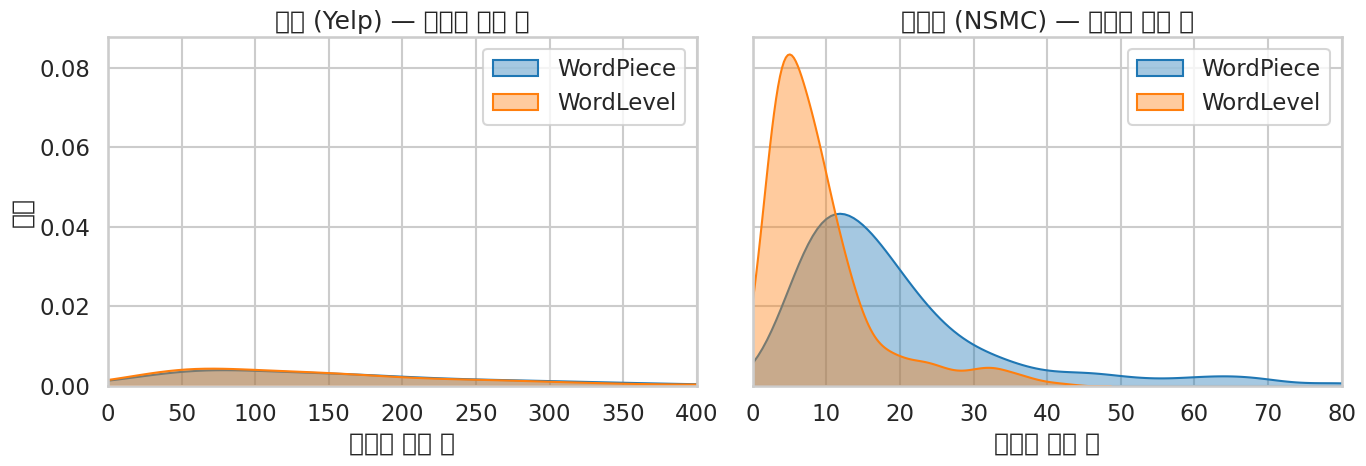
\includegraphics[width=0.92\linewidth]{assets/figures/ch19_token_length_distribution.png}
\end{bookfigurelabel}

\textbf{그림 읽기} --- 그림~\ref{fig:ch19-token-length-distribution}에서 다음 내용을 확인합니다: WordPiece와 WordLevel의 문장당 토큰 수 분포. 실행된 노트북에서 저장된 최신 plot 출력이므로, 코드에서 계산한 값이 어떤 평가 지점으로 이어지는지 바로 확인할 수 있습니다.



\textbf{해석}

\begin{itemize}
\tightlist
\item
  영어에서는 \emph{WordPiece 가 WordLevel 보다 토큰 수가 살짝 더 많음} --- subword 분할로 한 단어가 여러 조각으로 쪼개지기 때문. 하지만 \texttt{{[}UNK{]}} 가 거의 안 생기는 \emph{대가} 로 받아들이는 trade-off.
\item
  한국어에서는 \emph{WordLevel 의 평균 토큰 수가 매우 작아 보이지만} (어절 단위), 다음 §5-2 의 UNK 비율을 보면 그 \emph{대가} 가 드러납니다.
\end{itemize}



\subsection{미등록 토큰 비율}

같은 eval 코퍼스에서 각 토크나이저가 \emph{얼마나 자주} \texttt{{[}UNK{]}} 를 출력하는지. WordPiece 의 \emph{진짜 장점} 이 여기서 드러납니다.



\Needspace{10\baselineskip}
\begin{lstlisting}
def unk_rate(tok, texts):
    total_tokens = 0
    unk_tokens = 0
    for t in texts:
        toks = tok.encode(t).tokens
        total_tokens += len(toks)
        unk_tokens += sum(1 for tk in toks if tk == "[UNK]")
    return unk_tokens / total_tokens if total_tokens > 0 else 0.0

\end{lstlisting}

\noindent\emph{앞 블록은 앞에서 만든 중간 값을 다음 계산으로 넘기는 단계입니다. 이어지는 블록에서는 텍스트를 모델 입력 텐서로 바꾸는 단계로 넘어갑니다.}

\Needspace{11\baselineskip}
\begin{lstlisting}[firstnumber=10]
unk_summary = pd.DataFrame({
    "tokenizer": ["en WordPiece", "en WordLevel", "ko WordPiece", "ko WordLevel"],
    "unk_rate": [
        unk_rate(tok_en_wp, eval_en),
        unk_rate(tok_en_wl, eval_en),
        unk_rate(tok_ko_wp, eval_ko),
        unk_rate(tok_ko_wl, eval_ko),
    ],
})
unk_summary["unk_pct"] = unk_summary["unk_rate"].apply(lambda x: f"{x:.2%}")
print(
    unk_summary[["tokenizer", "unk_pct"]].to_string(index=False)
)
\end{lstlisting}



\compactCodeOmitted{텍스트를 모델 입력 텐서로 바꾸는 단계}

\begin{bookfigurelabel}[H]{토크나이저별 미등록 토큰 비율 비교}{fig:ch19-unk-rate-bar}
\centering
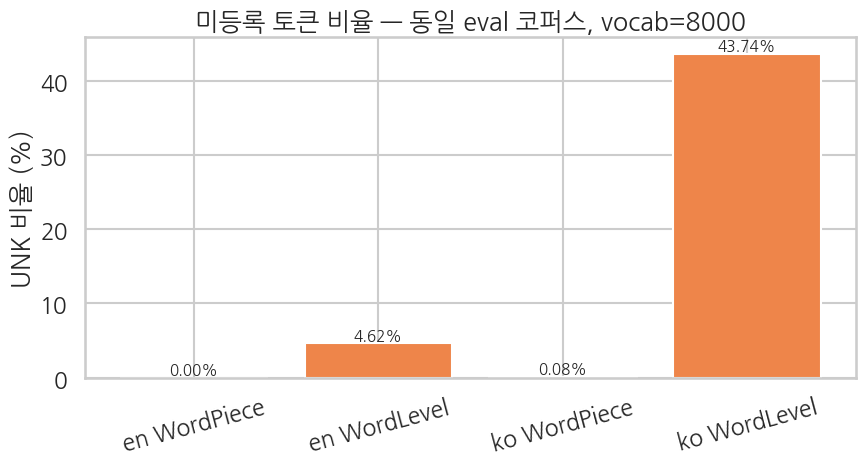
\includegraphics[width=0.72\linewidth]{assets/figures/ch19_unk_rate_bar.png}
\end{bookfigurelabel}

\textbf{그림 읽기} --- 그림~\ref{fig:ch19-unk-rate-bar}에서 다음 내용을 확인합니다: 토크나이저별 미등록 토큰 비율 비교. 실행된 노트북에서 저장된 최신 plot 출력이므로, 코드에서 계산한 값이 어떤 평가 지점으로 이어지는지 바로 확인할 수 있습니다.



\textbf{해석 --- 이 장의 가장 중요한 결과}

\begin{itemize}
\tightlist
\item
  \textbf{WordPiece (양쪽 언어 모두)}: UNK 비율 거의 0\%. \emph{모르는 단어} 가 와도 작은 조각으로 분해 가능.
\item
  \textbf{WordLevel (영어)}: 보통 1-3\% --- 영어는 어휘가 한정되어 8K vocab 으로도 그럭저럭 커버.
\item
  \textbf{WordLevel (한국어)}: 5-15\% --- 교착어 특성상 \emph{같은 어근의 다른 활용} 이 vocab 을 잡아먹어 vocab 부족.
\end{itemize}

\begin{quote}
\textbf{BERT 가 WordPiece 를 채택한 이유} --- 모든 단어가 \emph{학습 가능한 표현} 으로 인코딩되어, 모델이 가지런한 임베딩 공간에서 작동할 수 있음. WordLevel 처럼 \texttt{{[}UNK{]}} 가 빈번하면 그 위치들은 \emph{학습 신호가 사라진 빈 구멍} 이 됩니다.
\end{quote}



\subsection{\texorpdfstring{2\(\times\)2 비교 표 --- 한눈에 정리}{2\textbackslash times2 비교 표 --- 한눈에 정리}}

같은 vocab=8000 일 때 \emph{언어 \(\times\) 알고리즘} 의 모든 조합.



\subsection{교차 언어 적용}

지금까지 \emph{학습 언어 = 적용 언어} 였습니다. 만약 \textbf{다른 언어 텍스트} 를 학습한 토크나이저에 통과시키면?

\begin{itemize}
\tightlist
\item
  \textbf{WordPiece (영어)} \(\to\) 한국어 텍스트: 한국어 글자가 vocab 에 없어 대부분 \textbf{\texttt{{[}UNK{]}} 로 떨어짐} (BERT character fallback 도 없으면)
\item
  \textbf{WordLevel (영어)} \(\to\) 한국어 텍스트: 한국어 \emph{어절 통째} 가 단어로 vocab 에 없어 \textbf{거의 100\% UNK}
\item
  반대 (한국어 학습 \(\to\) 영어 입력) 도 같은 양상
\end{itemize}

이걸 정량 비교하면 “왜 multilingual 모델은 \emph{공통 vocab} (mBERT 의 110k WordPiece, XLM-R 의 250k SentencePiece) 으로 학습되는지” 가 직관됩니다.



\Needspace{11\baselineskip}
\begin{lstlisting}
tokenizers = {
    "en_WordPiece": tok_en_wp,
    "en_WordLevel": tok_en_wl,
    "ko_WordPiece": tok_ko_wp,
    "ko_WordLevel": tok_ko_wl,
}

cross_examples = [
    ("EN", "The food was absolutely delicious and the service was great."),
    ("KO", "음식이 정말 맛있었고 서비스도 훌륭했습니다."),
]

\end{lstlisting}

\noindent\emph{앞뒤 블록은 모두 텍스트를 모델 입력 텐서로 바꾸는 단계입니다. 길이를 나누어 같은 흐름을 단계별로 확인합니다.}

\Needspace{11\baselineskip}
\begin{lstlisting}[firstnumber=13]
cross_rows = []
for lang, text in cross_examples:
    for tok_name, tok in tokenizers.items():
        enc = tok.encode(text)
        n_tokens = len(enc.tokens)
        n_unk = sum(1 for t in enc.tokens if t == "[UNK]")
        cross_rows.append({
            "input_lang": lang,
            "tokenizer": tok_name,
            "tokenizer_train_lang": "EN" if "en_" in tok_name else "KO",
            "n_tokens": n_tokens,
            "n_unk": n_unk,
            "unk_pct": round(n_unk / n_tokens * 100, 1) if n_tokens else 0.0,
            "match": "OK same" if (lang.lower() in tok_name.lower()[:5]) else "X cross",
        })

\end{lstlisting}

\noindent\emph{앞 블록은 텍스트를 모델 입력 텐서로 바꾸는 단계입니다. 이어지는 블록에서는 앞에서 만든 중간 값을 다음 계산으로 넘기는 단계로 넘어갑니다.}

\Needspace{5\baselineskip}
\begin{lstlisting}[firstnumber=29]
cross_df = pd.DataFrame(cross_rows)
print(cross_df.to_string(index=False))
\end{lstlisting}

\begin{codeRead}
\textbf{1--6행}의 \inlinecode{tokenizers = ...}에서는 이후 분석에서 사용할 값을 준비합니다. \textbf{8--11행}의 \inlinecode{cross\_examples = ...}에서는 이후 분석에서 사용할 값을 준비합니다. \textbf{13행}의 \inlinecode{cross\_rows = ...}에서는 이후 분석에서 사용할 값을 준비합니다.
\end{codeRead}



\Needspace{11\baselineskip}
\begin{lstlisting}
print("=" * 78)
for lang, text in cross_examples:
    print(f"\n[input ({lang})]  {text}")
    for tok_name, tok in tokenizers.items():
        enc = tok.encode(text)
        cross = "X" if (lang.lower()[:2] not in tok_name.lower()[:5]) else "  "
        head = enc.tokens[:12]
        print(
            f"  {cross} {tok_name:18} ({len(enc.tokens):>3} tokens, UNK {sum(1 for t in enc.tokens if t=='[UNK]'):>2}): "
            f"{head}"
        )
\end{lstlisting}

\begin{codeRead}
\textbf{2행}의 \inlinecode{for lang, text in cross\_e...}에서는 앞 단계에서 만든 값을 바탕으로 다음 계산을 수행합니다. \textbf{4행}의 \inlinecode{for tok\_name, tok in toke...}에서는 앞 단계에서 만든 값을 바탕으로 다음 계산을 수행합니다. \textbf{5행}의 \inlinecode{enc = ...}에서는 이후 분석에서 사용할 값을 준비합니다.
\end{codeRead}



\compactCodeOmitted{텍스트를 모델 입력 텐서로 바꾸는 단계}

\begin{bookfigurelabel}[H]{학습 언어와 입력 언어가 다를 때의 미등록 토큰 비율}{fig:ch19-cross-language-heatmap}
\centering
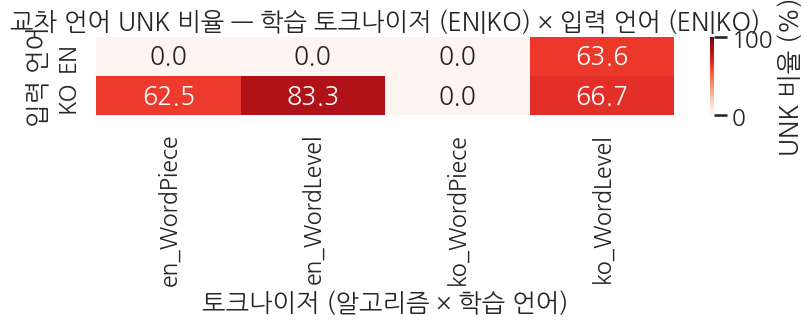
\includegraphics[width=0.78\linewidth]{assets/figures/ch19_cross_language_heatmap.png}
\end{bookfigurelabel}

\textbf{그림 읽기} --- 그림~\ref{fig:ch19-cross-language-heatmap}에서 다음 내용을 확인합니다: 학습 언어와 입력 언어가 다를 때의 미등록 토큰 비율. 실행된 노트북에서 저장된 최신 plot 출력이므로, 코드에서 계산한 값이 어떤 평가 지점으로 이어지는지 바로 확인할 수 있습니다.



\textbf{관찰}

\begin{itemize}
\tightlist
\item
  대각선(같은 언어) 셀은 UNK 가 거의 0 --- 학습 언어와 같으면 vocab 이 커버.
\item
  \textbf{비대각선(교차) 셀은 UNK 가 크게 솟음} --- 특히 WordLevel 은 어절 매칭이라 \emph{거의 100\%}, WordPiece 는 서브워드라도 한·영 \emph{글자} 가 vocab 에 없으면 통째 UNK.
\item
  WordPiece 가 그나마 한·영 \emph{공통 알파벳·구두점} 일부를 커버할 수 있지만, \emph{한글 자모/조합} 또는 \emph{영문 단어} 자체는 학습 corpus 에 의존.
\end{itemize}

\textbf{시사점}

\begin{itemize}
\tightlist
\item
  \textbf{단일 언어 corpus 로 학습한 토크나이저는 다른 언어에 거의 못 씁니다.} 모델을 통째 다른 언어로 재사용하려면 \emph{vocab 부터} 그 언어 데이터를 보고 학습해야 합니다.
\item
  \textbf{multilingual 모델} (mBERT, XLM-R, mT5 등)은 \emph{수십-백여 언어 corpus 를 섞어} 토크나이저를 학습해 \emph{공통 vocab} 을 만듭니다 --- 그래서 한 모델로 여러 언어 입력이 가능.
\item
  \textbf{byte-level BPE} (GPT-2/RoBERTa) 나 \textbf{SentencePiece(Unigram)} (T5/Llama) 같은 \emph{byte/character 단위 fallback} 이 있는 토크나이저는 UNK 가 원리상 없습니다 --- 단 비-학습 언어는 \emph{매우 긴 토큰 시퀀스} 가 되어 비효율적.
\end{itemize}

\begin{quote}
즉 “토크나이저는 모델의 언어를 \emph{물리적으로 결정} 한다” 가 이 장의 큰 결론. \ref{ch:20}--\ref{ch:23}장에서 사전학습 모델의 토크나이저 (\inlinecode{bert-base-uncased} / \inlinecode{klue/bert-base}) 를 그대로 가져오는 이유 --- 모델 본체와 \emph{vocab 일치} 가 필수.
\end{quote}



\section{\texorpdfstring{저장과 로드}{저장과 로드}}

토크나이저는 학습 후 \emph{파일로 저장} 해 다음 장에서 불러 쓸 수 있어야 합니다. HF 인터페이스 (\inlinecode{AutoModel.from\_pretrained} 와 함께 사용 가능한 형태) 로 wrap 하는 패턴도 시연.



\Needspace{11\baselineskip}
\begin{lstlisting}
import os
os.makedirs("./tokenizers_ch19", exist_ok=True)

tok_en_wp.save("./tokenizers_ch19/en_wordpiece.json")
tok_ko_wp.save("./tokenizers_ch19/ko_wordpiece.json")
tok_en_wl.save("./tokenizers_ch19/en_wordlevel.json")
tok_ko_wl.save("./tokenizers_ch19/ko_wordlevel.json")

print("saved 4 tokenizer files:")
for p in sorted(os.listdir("./tokenizers_ch19")):
    size_kb = os.path.getsize(f"./tokenizers_ch19/{p}") / 1024
    print(f"  ./tokenizers_ch19/{p}  ({size_kb:.1f} KB)")
\end{lstlisting}



\Needspace{8\baselineskip}
\begin{lstlisting}
tok_en_wp_loaded = Tokenizer.from_file("./tokenizers_ch19/en_wordpiece.json")
enc_orig = tok_en_wp.encode(SAMPLE_EN).tokens
enc_loaded = tok_en_wp_loaded.encode(SAMPLE_EN).tokens
print(f"original tokens : {enc_orig}")
print(f"loaded tokens   : {enc_loaded}")
print(f"match           : {enc_orig == enc_loaded}")
\end{lstlisting}



\Needspace{11\baselineskip}
\begin{lstlisting}
hf_en_wp = PreTrainedTokenizerFast(
    tokenizer_object=tok_en_wp,
    unk_token="[UNK]",
    pad_token="[PAD]",
    cls_token="[CLS]",
    sep_token="[SEP]",
    mask_token="[MASK]",
)

print(f"vocab_size      : {hf_en_wp.vocab_size}")
print(f"pad_token_id    : {hf_en_wp.pad_token_id}")
print(f"cls_token_id    : {hf_en_wp.cls_token_id}")

\end{lstlisting}

\noindent\emph{앞 블록은 텍스트를 모델 입력 텐서로 바꾸는 단계입니다. 이어지는 블록에서는 앞에서 만든 중간 값을 다음 계산으로 넘기는 단계로 넘어갑니다.}

\Needspace{11\baselineskip}
\begin{lstlisting}[firstnumber=14]
enc = hf_en_wp(
    SAMPLE_EN,
    padding=True,
    truncation=True,
    max_length=32,
    return_tensors="pt",
)
print(f"\ninput_ids shape : {enc['input_ids'].shape}")
print(f"input_ids       : {enc['input_ids'][0].tolist()}")
print(
    f"decoded         : "
    f"{hf_en_wp.decode(enc['input_ids'][0])}"
)
\end{lstlisting}

\noindent\textbf{출력.}
\begin{bookoutputbox}
vocab_size      : 8000
pad_token_id    : 0
cls_token_id    : 2

input_ids shape : torch.Size([1, 15])
input_ids : [2, 107, 218, 128, 4814, 5350, 3763, 300, 115, 107, 312, 128, 9...
decoded : [CLS] the food was unforgettable and the service was excellent. [...
\end{bookoutputbox}
\par\vspace{0.9em}



\begin{previewBox}{미리보기}
\textbf{다음 장의 다리} --- \ref{ch:20}장부터는 이 wrap 패턴으로 토크나이저를 모델에 연결합니다. 단, \emph{학습 안정성} 을 위해 \ref{ch:20}장+ 는 \emph{직접 학습한 토크나이저 대신} 표준 사전학습 토크나이저 (\inlinecode{bert-base-uncased}, \inlinecode{klue/bert-base}) 를 가져옴 --- \ref{ch:19}장의 \emph{경험} 위에 표준 도구의 신뢰성을 얹는 구조.
\end{previewBox}



\section{변형: 어휘 수 스윕}

\inlinecode{vocab\_size} 를 1K / 4K / 8K / 16K 로 sweep 하며 영어 WordPiece 의 mean 토큰 수와 UNK 비율이 어떻게 변하는지. vocab 이 \emph{작을수록} 토큰 수는 늘고, \emph{클수록} 토큰 수는 줄지만 vocab 자체가 무거워짐 --- 모델 크기와의 trade-off.



\compactCodeOmitted{숫자 결과를 그림으로 확인하는 단계}

\begin{bookfigurelabel}[H]{WordPiece 어휘 수에 따른 토큰 길이와 미등록 토큰 비율}{fig:ch19-vocab-sweep}
\centering
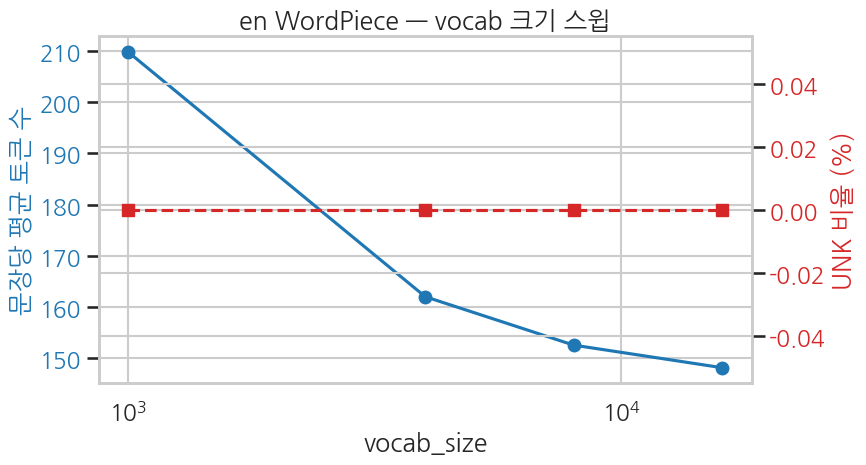
\includegraphics[width=0.78\linewidth]{assets/figures/ch19_vocab_sweep.png}
\end{bookfigurelabel}

\textbf{그림 읽기} --- 그림~\ref{fig:ch19-vocab-sweep}에서 다음 내용을 확인합니다: WordPiece 어휘 수에 따른 토큰 길이와 미등록 토큰 비율. 실행된 노트북에서 저장된 최신 plot 출력이므로, 코드에서 계산한 값이 어떤 평가 지점으로 이어지는지 바로 확인할 수 있습니다.



\textbf{해석}

\begin{itemize}
\tightlist
\item
  vocab 1K --- 극단적인 subword 분할 (한 단어 = 5+ 조각), UNK 는 거의 없음.
\item
  vocab 8K-16K --- 한 단어가 보통 1-2 조각으로 안정. UNK 는 거의 0\%.
\item
  표준 BERT (vocab 30K) 는 이 curve 의 \emph{오른쪽 끝} --- 한 단어가 거의 1 토큰에 수렴.
\end{itemize}

\begin{quote}
\textbf{실무 가이드} --- 사전학습 BERT 와 같은 \emph{모델 크기} 를 노린다면 vocab 30K, 작은 모델 (\ref{ch:20}장의 scratch BERT) 이면 8K-16K 가 적절. vocab 이 커지면 임베딩 테이블 파라미터도 커지니 (\(V \times H\)) 모델 전체 크기와 함께 결정해야 합니다.
\end{quote}



\section{이 장에 등장한 라이브러리·함수}

\begin{booktable}{19장 새로 등장한 라이브러리}{tab:ch19-04}
\begin{adjustbox}{max width=\textwidth}
\begin{tabular}{@{}lll@{}}
\toprule
이름 & 한 줄 설명 & 다음 장에서 \\
\midrule

\inlinecode{tokenizers.Tokenizer} & 학습·인코딩의 최상위 컨테이너 & \ref{ch:20}장+ 는 사전학습 토크나이저를 \inlinecode{AutoTokenizer} 로 받음 \\
\inlinecode{tokenizers.models.WordPiece} & BERT 표준 subword 모델 & (동일 알고리즘이 BERT 사전학습에 사용) \\
\inlinecode{tokenizers.models.WordLevel} & 어절 단위 (비교용) & \ref{ch:19}장 한정 \\
\inlinecode{tokenizers.trainers.WordPieceTrainer} & likelihood 기반 vocab 학습 & 같음 \\
\inlinecode{tokenizers.pre\_tokenizers.BertPreTokenizer} & BERT 표준 공백·구두점 분할 & 같음 \\
\inlinecode{tokenizers.processors.TemplateProcessing} & \texttt{{[}CLS{]}\ /\ {[}SEP{]}} 자동 부착 & \ref{ch:20}장+ MLM 입력 포맷 \\
\inlinecode{transformers.PreTrainedTokenizerFast} & HF 표준 인터페이스로 wrap & \ref{ch:20}장에서 표준 패턴 \\
\bottomrule
\end{tabular}
\end{adjustbox}
\end{booktable}



\section{체크포인트 질문}

\begin{enumerate}
\def\labelenumi{\arabic{enumi}.}
\tightlist
\item
  WordPiece 의 \inlinecode{\#\#} prefix 가 의미하는 바는 무엇이고, WordLevel 토크나이저에는 왜 \inlinecode{\#\#} 토큰이 0 개인가요?
\item
  같은 vocab 크기 (8K) 에서 한국어 WordLevel 의 UNK 비율이 영어 WordLevel 보다 \emph{훨씬} 높은 이유 두 가지를 들어보세요.
\item
  vocab 크기를 키우면 mean 토큰 수는 줄고 UNK 비율도 줄어드는데, 왜 BERT 의 표준 vocab 이 무한대가 아니라 30K 정도인가요?
\item
  \inlinecode{unforgettable} 이 학습 코퍼스에 \emph{없는} 단어일 때, WordPiece 와 WordLevel 이 각각 어떻게 처리하나요?
\end{enumerate}



\section{FAQ}

\begin{faqBox}{Q1. (이론) WordPiece 와 BPE 는 무엇이 다른가요?}

알고리즘 \emph{흐름} 은 거의 같습니다 --- 둘 다 \emph{문자 단위 vocab} 에서 시작해 자주 등장하는 \emph{조각 쌍} 을 병합하며 vocab 을 키웁니다. 차이는 \emph{어떤 쌍을 병합할지} 의 기준:

\begin{itemize}
\tightlist
\item
  \textbf{BPE} (GPT 시리즈): 단순히 \emph{코퍼스에서 가장 빈번한} 쌍을 병합 (frequency-based).
\item
  \textbf{WordPiece} (BERT 시리즈): \emph{언어 모델 likelihood 가 가장 많이 오르는} 쌍을 병합 (likelihood-based). 식: \(\text{score} = \dfrac{\text{count}(AB)}{\text{count}(A) \cdot \text{count}(B)}\).
\end{itemize}

실무적 차이는 \emph{작아} 두 알고리즘의 토큰화 결과가 비슷한 경우가 많습니다. \ref{ch:24}장 (GPT prototype) 에서 BPE 를 직접 다룹니다.

\end{faqBox}

\begin{faqBox}{Q2. (실무) \inlinecode{vocab\_size} 를 8K 로 잡았는데 BERT 표준 30K 와 무엇이 다른가요?}

vocab 이 작으면 \emph{한 단어가 여러 조각} 으로 더 잘게 쪼개져 sequence 길이가 길어집니다. 길어진 sequence 는 attention 비용 (\(O(n^2)\)) 을 늘려 학습이 \emph{느려짐}. 반대로 vocab 이 크면 \emph{임베딩 테이블} 자체가 커져 모델 파라미터가 늘어남 (\(V \times H\), BERT-base 면 \(30000 \times 768 \approx 23M\)).

실무 trade-off --- 모델이 작을수록 (이 장 다음 \ref{ch:20}장처럼 \emph{scratch} 작은 BERT) 작은 vocab (8K-16K) 이 합리적, 큰 모델은 큰 vocab (30K-50K) 이 안정적.

\Needspace{5\baselineskip}
\begin{lstlisting}
vocab_size = 8000
hidden = 256
embed_params = vocab_size * hidden  # = 2.05M
\end{lstlisting}

\end{faqBox}


\begin{faqBox}{Q4. (실무) 의료·법률 같은 \emph{전문 도메인} 에서 직접 학습한 토크나이저는 얼마나 효과적인가요?}

전문 도메인 어휘는 일반 위키·뉴스 코퍼스에 거의 없어서 표준 BERT 토크나이저는 그 단어들을 \emph{너무 잘게} 쪼갭니다. 예: \inlinecode{corticosteroid} \(\to\) \inlinecode{cor}, \inlinecode{\#\#ti}, \inlinecode{\#\#co}, \inlinecode{\#\#ster}, \inlinecode{\#\#oid} (5 토큰). 도메인 코퍼스로 직접 학습하면 \inlinecode{corticosteroid} 가 1 토큰으로 들어가 (a) 입력이 짧아져 학습 빠름 (b) 모델이 \emph{의미 단위} 로 학습 --- BioBERT, LegalBERT 같은 도메인 모델이 모두 이 패턴.

도메인 코퍼스가 1GB+ 정도 모이면 (\inlinecode{vocab\_size=20000-30000}) 직접 학습할 가치가 있습니다.

\end{faqBox}






\compactFAQMore{4}

\begin{previewBox}{미리보기: 다음 장}

\textbf{\ref{ch:20}장. 작은 BERT 직접 사전학습 (영어 MLM)}

\begin{itemize}
\tightlist
\item
  이 장에서 \emph{경험한} 토크나이저 학습 위에, \emph{모델 자체} 를 from-scratch 로 사전학습.
\item
  모델: 작은 BERT (n\_layer=4, hidden=256) --- \inlinecode{BertConfig} 로 직접 설계.
\item
  토크나이저: 표준 \inlinecode{bert-base-uncased} 의 WordPiece 를 가져옴 (학습 안정성 우선).
\item
  데이터: \inlinecode{yelp\_polarity} 의 text (라벨 무시) --- \emph{MLM} 사전학습.
\item
  Loss: \inlinecode{CrossEntropyLoss} (마스킹된 위치의 토큰 예측).
\item
  \ref{ch:21}장에서 이 사전학습 모델로 Yelp 이진 분류 \(\to\) \ref{ch:10}장 (DistilBERT 사전학습) 과 \emph{직접 비교} --- \emph{직접 사전학습한 작은 BERT} 가 \emph{대규모 사전학습된 DistilBERT} 와 얼마나 차이 나는지.
\end{itemize}

\begin{quote}
\textbf{변하는 축}: Phase 3 안에서 \emph{모델 학습 task 가 등장} --- 사전학습 (MLM) 이라는 \emph{새로운 학습 방식} 이 핵심.
\end{quote}
\end{previewBox}